\documentclass{article}
\usepackage[spanish]{babel}
\usepackage[utf8]{inputenc}
\usepackage{amsmath}
\usepackage{amssymb}
\usepackage{graphicx}
\usepackage{listings}
\usepackage{xcolor}
\usepackage{float}
\usepackage{hyperref}
\usepackage{textgreek}
\usepackage{geometry}[margin=1in]

% Configuración para listings (código)
\lstset{
    basicstyle=\ttfamily\small,
    keywordstyle=\color{blue},
    stringstyle=\color{red},
    commentstyle=\color{green!60!black},
    numbers=left,
    numberstyle=\tiny\color{gray},
    stepnumber=1,
    numbersep=5pt,
    backgroundcolor=\color{white},
    showspaces=false,
    showstringspaces=false,
    showtabs=false,
    frame=single,
    rulecolor=\color{black},
    tabsize=2,
    captionpos=b,
    breaklines=true,
    breakatwhitespace=true,
    escapeinside={\%*}{*)}
}

\begin{document}

\begin{titlepage}
  \centering
  
\includegraphics[width=0.25\textwidth]{ITBA_logo.png}\par\vspace{1cm}
  {\textsc{Instituto Tecnológico de Buenos Aires} \par}
    \vspace{1cm}
    {\Large \textsc{Trabajo Práctico 2}\par}
    \vspace{1.5cm}
    {\huge\bfseries Autómatas Celulares\par}
    \vspace{2cm}
    {\Large\itshape Candisano, Gonzalo - 62616\\
	  Neme, Emilio Pablo - 62601\\
	Quian Blanco, Francisco - 63006\par}
    \vfill
    Simulación de Sistemas - 72.25
    \vfill
    \noindent\textbf{Profesores} \\
Parisi, Daniel \\
Patterson, Germán Agustín \\
Salgado Corrado, Ariel Olaf \\
Wiebke, Lucas
\vfill
    {\large Segundo cuatrimestre 2025 - Grupo 12\par}
\end{titlepage}

\section{Introducción}
Este trabajo práctico se enfoca en la simulación de sistemas complejos mediante la implementación y el análisis de un modelo de agente autopropulsado \textit{off-lattice}, basado en los trabajos de Vicsek (y otros) [1] y Baglietto \& Vazquez [2].

\medskip

El objetivo central es estudiar el fenómeno de ordenamiento espontáneo y la transición de fase en un sistema de partículas que interactúan. Para ello, se implementa el modelo clásico de bandadas propuesto en [1], donde cada agente, caracterizado por su posición y velocidad, actualiza su dirección alineándose con la velocidad promedio de sus vecinos dentro de un radio de interacción, añadiendo además un ruido angular de amplitud $\eta$. El grado de orden del sistema se cuantifica mediante el observable de polarización ($v_a$).

\medskip

Posteriormente, se investiga una dinámica de interacción alternativa propuesta en [2], análoga a la de un modelo de votante. En esta variante, la regla de actualización se modifica: en lugar de promediar, cada partícula copia la dirección de velocidad de un único vecino seleccionado al azar dentro de su radio de interacción, sumando también una perturbación de ruido.

\medskip

El presente informe documenta el proceso de simulación, comenzando con la descripción del modelo y su implementación, seguido de los resultados organizados en: a) animaciones de la dinámica del sistema, b) evolución temporal de la polarización, c) curvas de \textit{input} (ruido $\eta$ y densidad $\rho$) vs. \textit{observable} ($v_a$) para ambos modelos, y d) el análisis comparativo de los resultados. Finalmente, se exponen las conclusiones sobre los comportamientos emergentes observados.

\section{Implementación}

\subsection{Descripción del Modelo de Vicsek}
El modelo implementado sigue la formulación de Vicsek (y otros). [1] para partículas autopropulsadas en un espacio bidimensional periódico de tamaño $L \times L$. Cada partícula $i$ está caracterizada por su posición $\vec{x_i}(t) = (x_i(t), y_i(t))$ y su dirección de movimiento $\theta_i(t)$, que evolucionan discretamente en el tiempo según las reglas:

\textbf{a) Actualización de posición:}
\begin{equation}
\vec{x_i}(t + \Delta t) = \vec{x_i}(t) + \vec{v_i}(t) \Delta t
\label{eq:posicion}
\end{equation}

donde $\vec{v_i}(t) = (v \cos \theta_i(t), v \sin \theta_i(t))$ es la velocidad de magnitud constante $v$. La posición se actualiza en cada paso temporal y se aplican condiciones de contorno periódicas.

\textbf{b) Actualización de dirección:}
Se implementaron dos reglas de alineamiento:
\begin{itemize}
\item \textbf{Modelo Clásico (Promedio) [1]:}
\begin{equation}
\theta_i(t + \Delta t) = \langle \theta_j(t) \rangle_{r} + \xi_i(t)
\label{eq:posicion}
\end{equation}
donde $\langle \cdot \rangle_{r}$ denota el promedio angular sobre todas las partículas $j$ (incluyendo a la propia partícula $i$) dentro de un radio de interacción $r$, y $\xi_i(t)$ es un ruido aleatorio uniformemente distribuido en $[-\eta/2, \eta/2]$.

\item \textbf{Modelo de Votante [2]:}
\begin{equation}
\theta_i(t + \Delta t) = \theta_k(t) + \xi_i(t)
\label{eq:posicion}
\end{equation}
donde $k$ es una partícula vecina elegida aleatoriamente (con igual probabilidad) de entre todas las partículas dentro del radio $r$ (incluyéndose a sí misma). $\xi_i(t)$ es el mismo ruido definido en el modelo clásico.
\end{itemize}

\textbf{c) Condiciones de contorno:} Se aplican condiciones periódicas en ambas direcciones para simular un sistema infinito:
\begin{equation}
x_i \leftarrow ((x_i \mod L) + L) \mod L, \quad y_i \leftarrow ((y_i \mod L) + L) \mod L
\label{eq:posicion}
\end{equation}

\subsection{Parámetros del Modelo}
Los principales parámetros del sistema y sus valores típicos o rangos de estudio son:
\begin{itemize}
\item $L$: Tamaño del espacio (longitud del lado del cuadrado). Valor por defecto: \textbf{10}.
\item $N$: Número de partículas. Valor por defecto: \textbf{300}.
\item $v$: Magnitud de la velocidad (constante para todas las partículas). Valor por defecto: \textbf{0.03}.
\item $r$: Radio de interacción. Valor por defecto: \textbf{1.0}.
\item $\eta$: Amplitud del ruido angular. Es la variable de control principal. Valor por defecto: \textbf{0.1}.
\item $\Delta t$: Paso temporal. Valor por defecto: \textbf{1}.
\item $\rho = N/L^2$: Densidad de partículas (parámetro derivado). Variable de estudio secundaria.
\end{itemize}

\subsection{Observable Principal: Polarización}
El grado de orden colectivo del sistema se cuantifica mediante el observable de \textbf{polarización $v_a$}, definido como el módulo del vector velocidad promedio normalizado:
\begin{equation}
v_a(t) = \frac{1}{N v} \left| \sum_{i=1}^{N} \vec{v_i}(t) \right| = \frac{1}{N} \left| \sum_{i=1}^{N} e^{i \theta_i(t)} \right|
\label{eq:posicion}
\end{equation}
donde $v_a \in [0, 1]$. Un valor $v_a \approx 1$ indica un alto grado de alineamiento y la formación de una bandada cohesionada, mientras que $v_a \approx 0$ corresponde a un movimiento desordenado y aleatorio de las partículas.

\subsection{Flujo de la Simulación}
El algoritmo avanza sincrónicamente en pasos de tiempo discretos. En cada iteración o paso $t$:
\begin{enumerate}
\item Para cada partícula, se determina su nuevo ángulo $\theta_i(t + \Delta t)$ según la regla de alineamiento seleccionada (promedio o votante) y el ruido aplicado.
\item Se actualiza la posición de cada partícula utilizando su nueva dirección.
\item Se aplican las condiciones de contorno periódicas a las nuevas posiciones.
\item El estado completo del sistema (x, y, $v_x$, $v_y$ de cada partcula) se escribe en un archivo de texto para su posterior análisis y visualización. Esta separación entre simulación y animación garantiza que la velocidad de visualización no dependa de la velocidad de cálculo del modelo.
\end{enumerate}

\section{Modelo}
El diagrama de clases UML (Figura 1) ilustra la estructura orientada a objetos del código implementado en Java. La simulación consta de:

\begin{itemize}
\item \textbf{Clase \texttt{Main}}: Punto de entrada del programa. Se encarga del parsing de argumentos de línea de comandos, la inicialización del modelo, y la ejecución del loop temporal principal que escribe los estados de las partículas en un archivo de texto.
\item \textbf{Clase \texttt{Vicsek}}: Constituye el núcleo del modelo. Implementa las reglas de actualización de posiciones y direcciones, la detección de vecinos dentro del radio de interacción, y los dos mecanismos de alineamiento (promedio y votante).
\item \textbf{Clase \texttt{Particle}}: Representa el estado de cada agente en el sistema, almacenando su posición (x, y), su dirección de movimiento (theta) y un identificador único (id).
\item \textbf{Clase \texttt{Config}}: Actúa como un contenedor para todos los parámetros de simulación (L, N, v, r, η, etc.), con valores por defecto definidos. Su propósito es organizar y facilitar el paso de estos parámetros a las demás clases.
\end{itemize}

\begin{figure}[H]
\centering
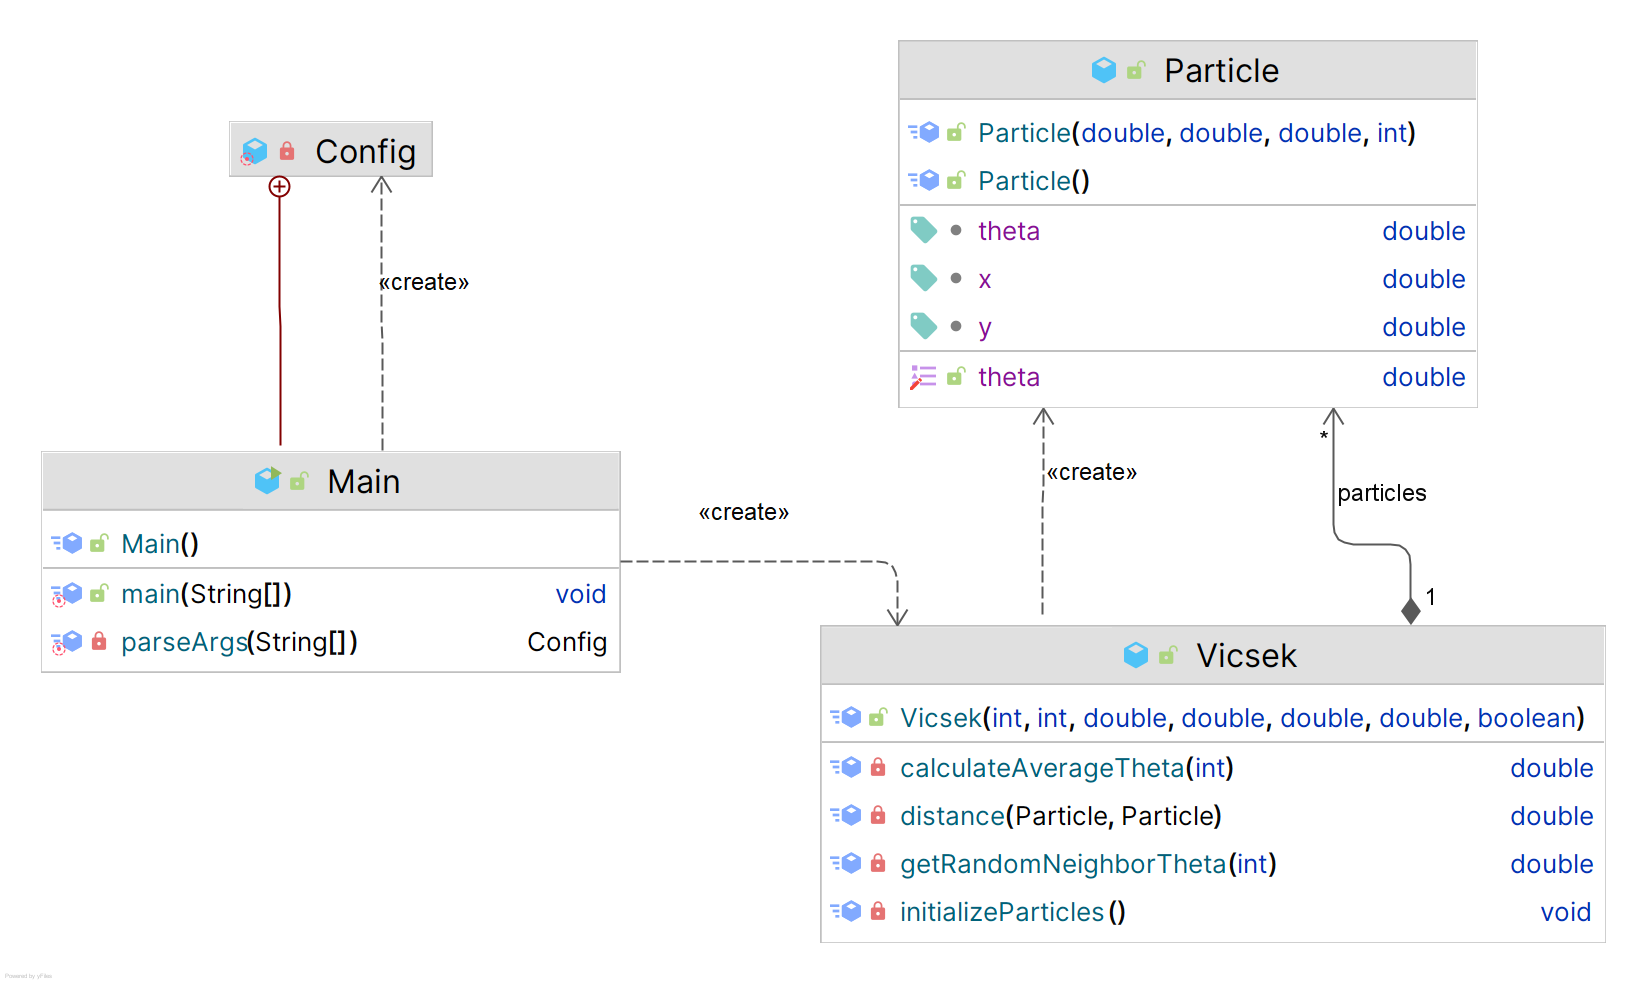
\includegraphics[width=0.9\textwidth]{TP2_UML.png}
\caption{Diagrama de clases UML de la implementación del modelo de Vicsek.}
\label{fig:uml}
\end{figure}

\section{Resultados}

Al analizar la evolución temporal de la polarización $v_a(t)$ observamos que, luego de un régimen transitorio inicial, el sistema alcanza un comportamiento estacionario. Este estado no implica necesariamente que $v_a(t)$ sea constante, sino que las fluctuaciones se estabilizan alrededor de un patrón característico para cada nivel de ruido $\eta$.  
A partir de la inspección de las curvas podemos identificar aproximadamente el momento en que se alcanza este régimen, y para el análisis descartamos los primeros pasos de simulación, promediando luego a partir del período estacionario para estimar el valor estacionario de $v_a$.

\subsection{Modelo Clásico de Vicsek}

\subsubsection{Dependencia con el Ruido $\eta$}
\begin{figure}[H]
\centering
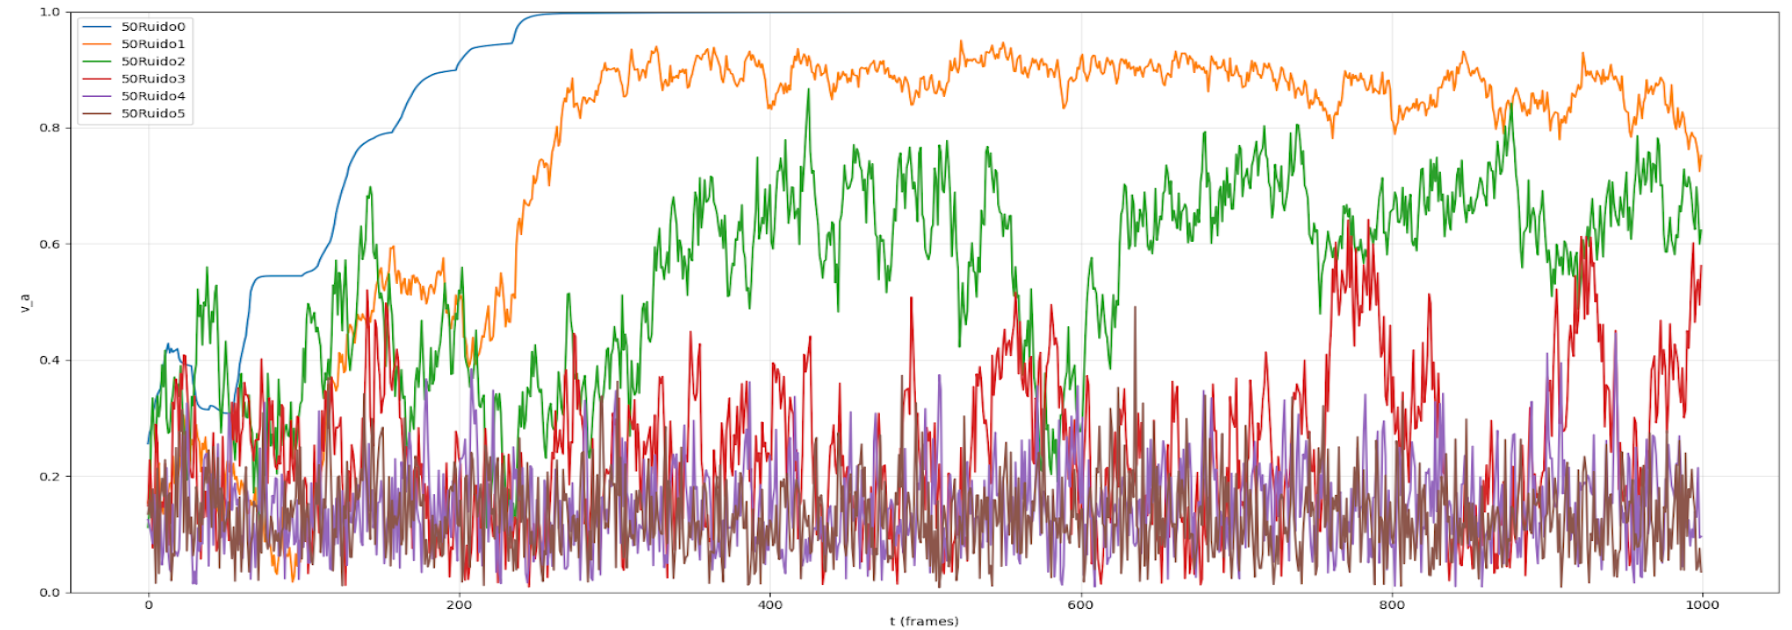
\includegraphics[width=0.9\textwidth]{polarizacion_vs_ruido_promedio.png}
\caption{Polarización $v_a$ en función del tiempo $t$ para el modelo clásico con $\rho = 0.5$ y $N = 50$, variando el ruido entre $\eta = 0$ y $\eta = 5$ }
\label{fig:va_vs_eta_promedio}
\end{figure}

\begin{figure}[H]
\centering
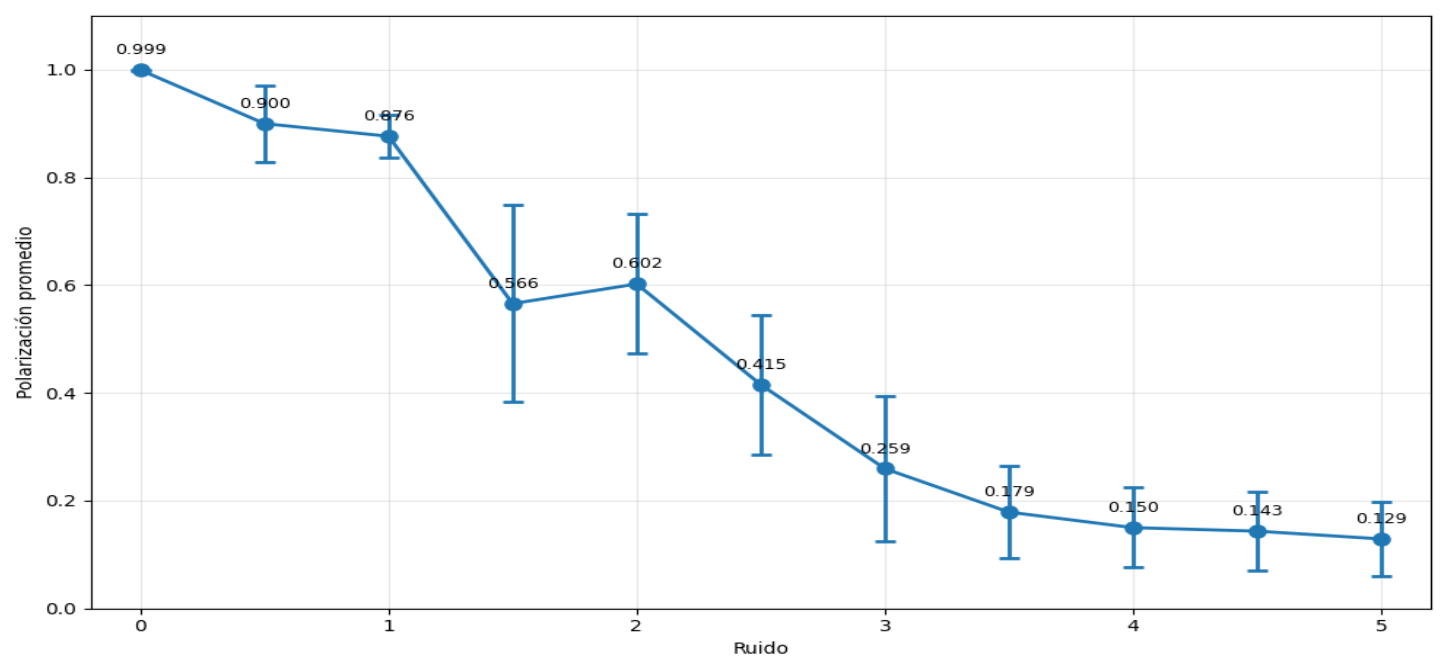
\includegraphics[width=0.9\textwidth]{polarizacion_vs_ruido_promedio2.png}
\caption{Valor promedio de la polarización en estado estacionario ($t=400$) en función del ruido $\eta$ ($N = 50$, $\rho = 10$).}
\label{fig:promedio_va_eta_promedio}
\end{figure}

\begin{figure}[H]
\centering
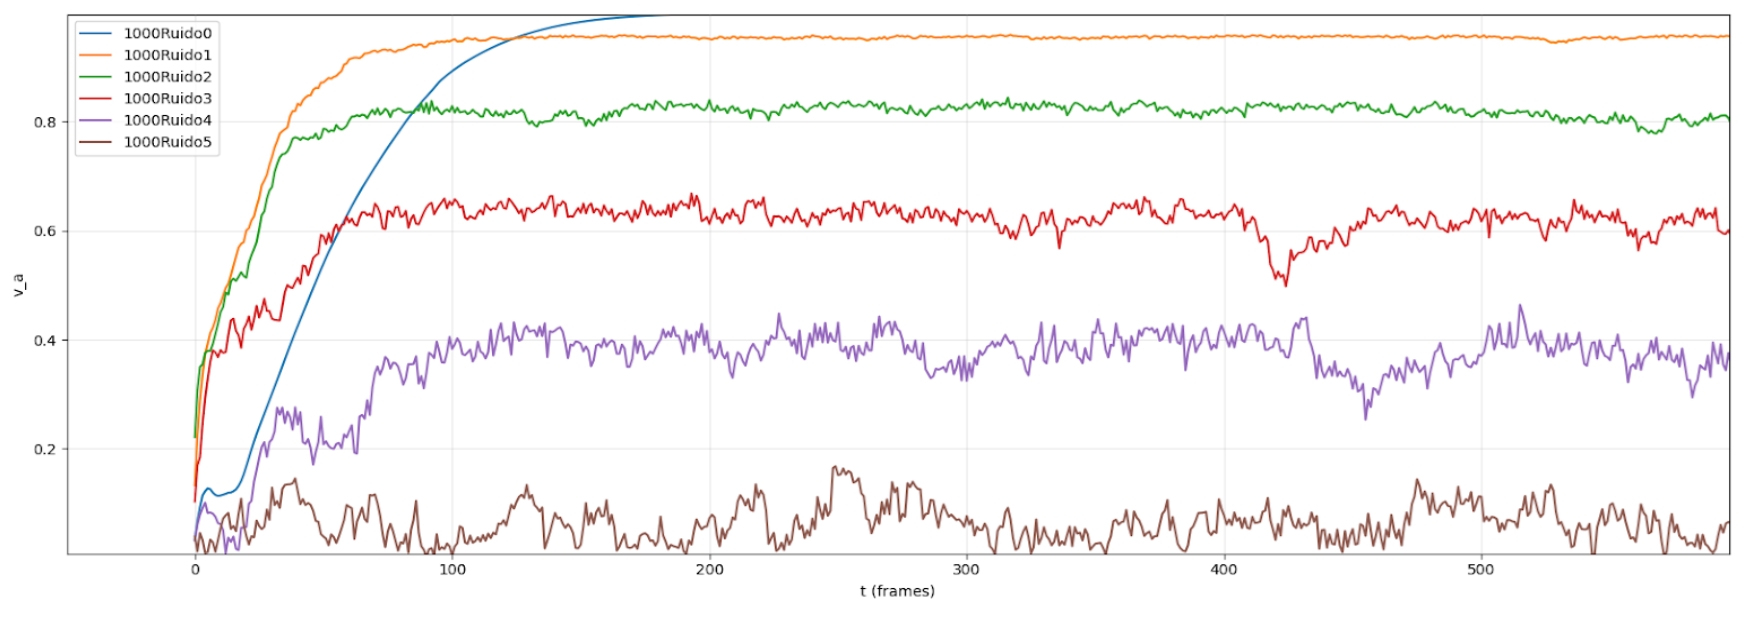
\includegraphics[width=0.9\textwidth]{promedio_polarizacion_ruido_promedio.png}
\caption{Polarización $v_a$ en función del tiempo $t$ para el modelo clásico con $\rho = 10$ y $N = 1000$, variando el ruido entre $\eta = 0$ y $\eta = 5$.}
\label{fig:va_vs_eta_promedio2}
\end{figure}

\begin{figure}[H]
\centering
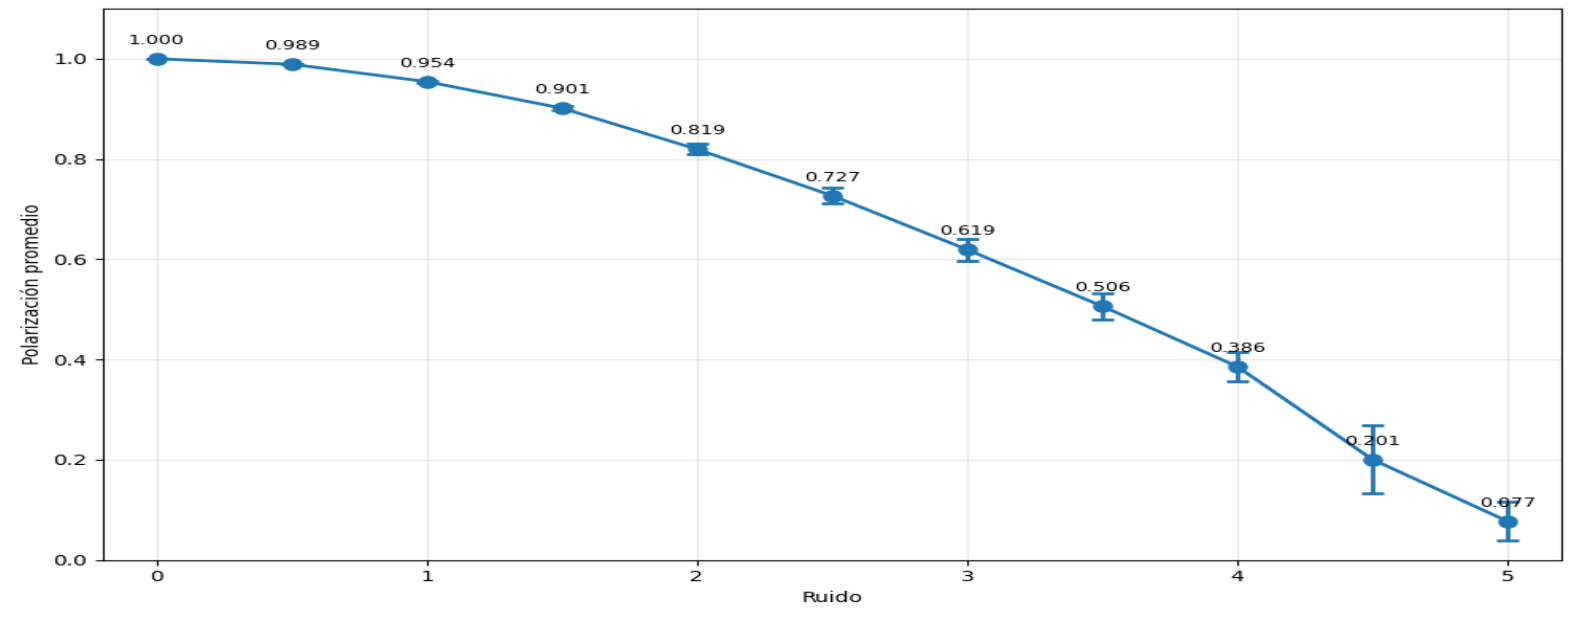
\includegraphics[width=0.9\textwidth]{promedio_polarizacion_ruido_promedio2.png}
\caption{Valor promedio de la polarización en estado estacionario ($t=200$) en función del ruido $\eta$ ($N = 1000$, $\rho = 10$).}
\label{fig:promedio_va_eta_promedio2}
\end{figure}

\subsubsection{Dependencia con la Densidad $\rho$}
\begin{figure}[H]
\centering
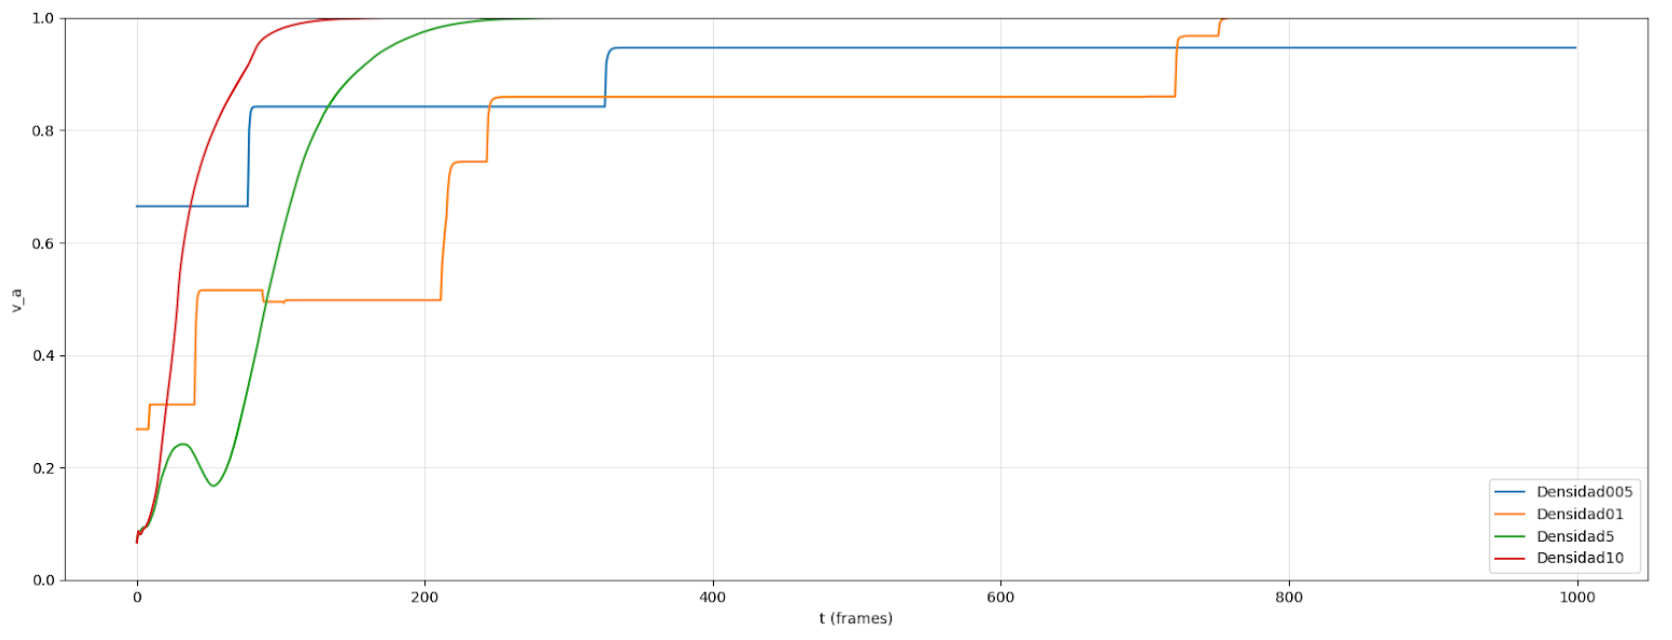
\includegraphics[width=0.9\textwidth]{17.png}
\caption{Polarización $v_a$ en función del tiempo $t$ para $\eta = 0$ variando N, para densidades de 0.5, 1, 5 y 10.}
\label{fig:17}
\end{figure}

\begin{figure}[H]
\centering
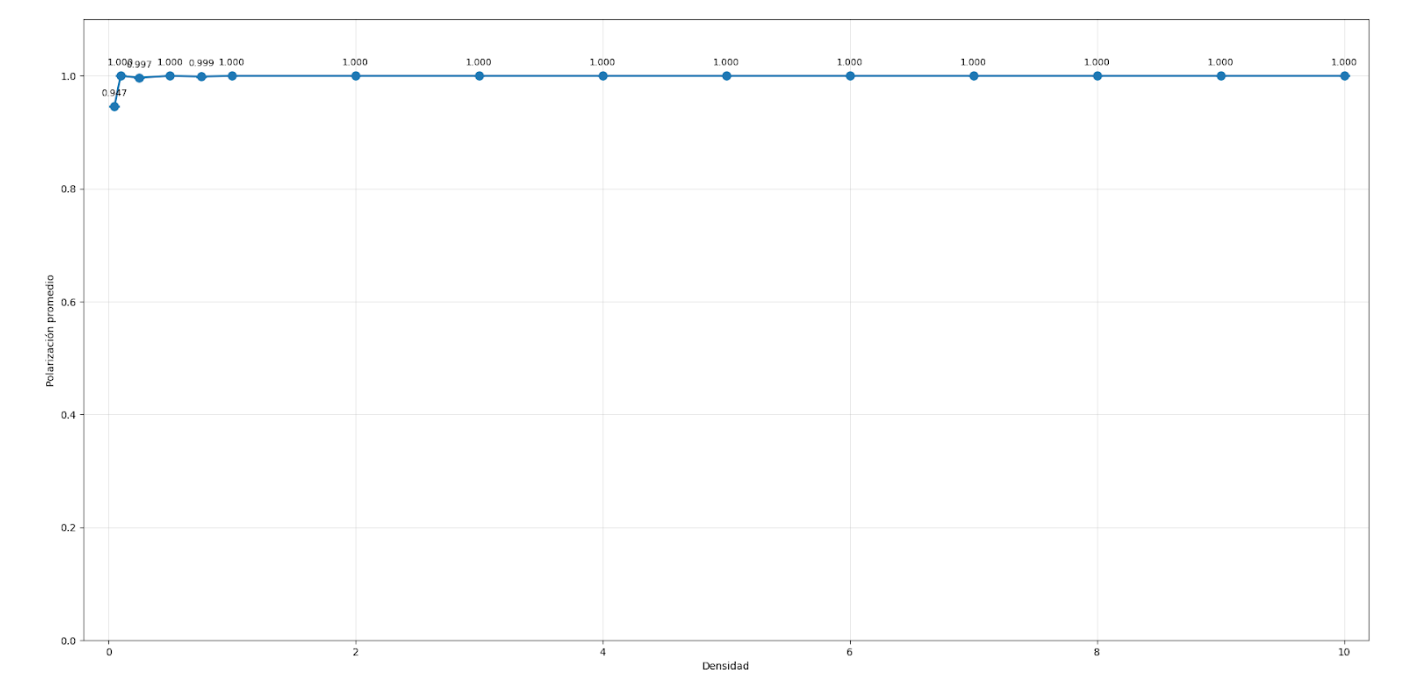
\includegraphics[width=0.9\textwidth]{18.png}
\caption{Valor promedio de la polarización en estado estacionario ($t = 800$) en función de la densidad $\rho$ para $\eta = 0$.}
\label{fig:18}
\end{figure}

\begin{figure}[H]
\centering
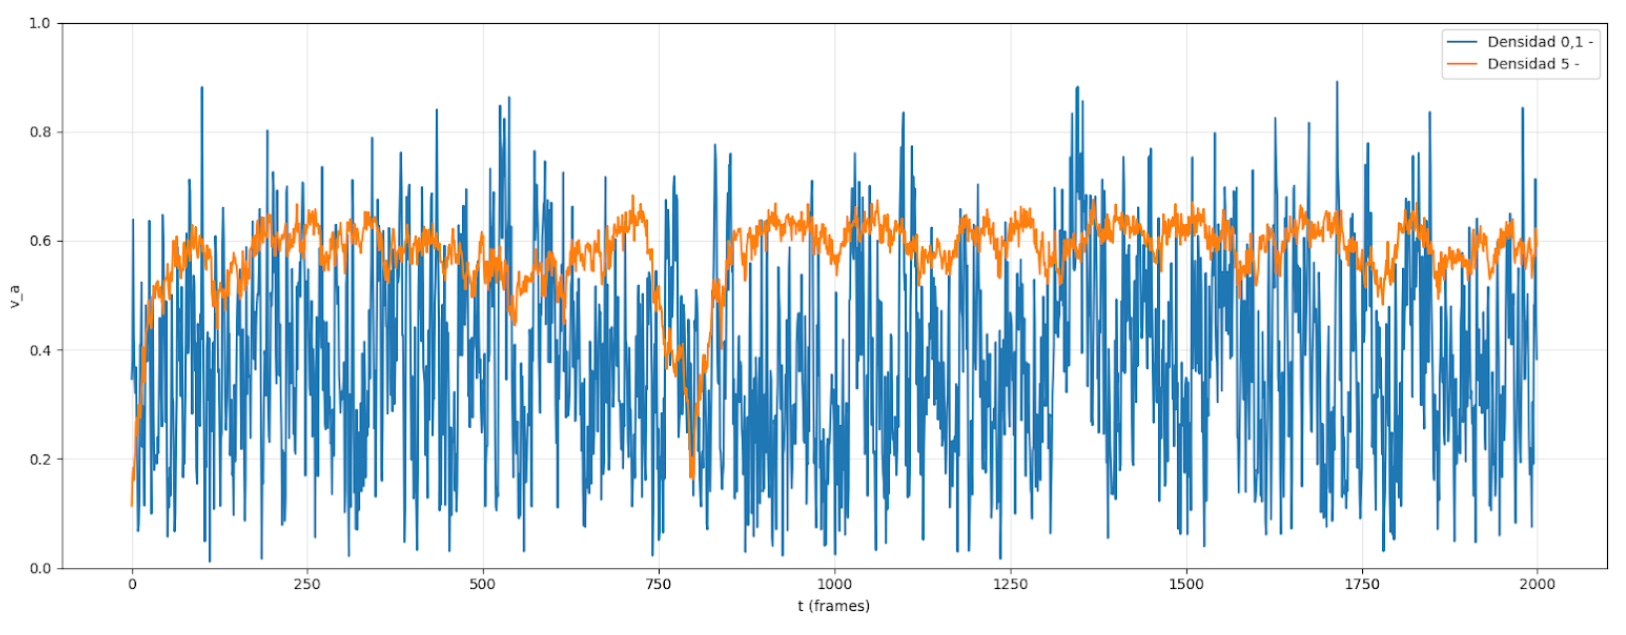
\includegraphics[width=0.9\textwidth]{19.png}
\caption{Polarización $v_a$ en función del tiempo $t$ para $\eta = 3$ variando densidad.}
\label{fig:19}
\end{figure}

\begin{figure}[H]
\centering
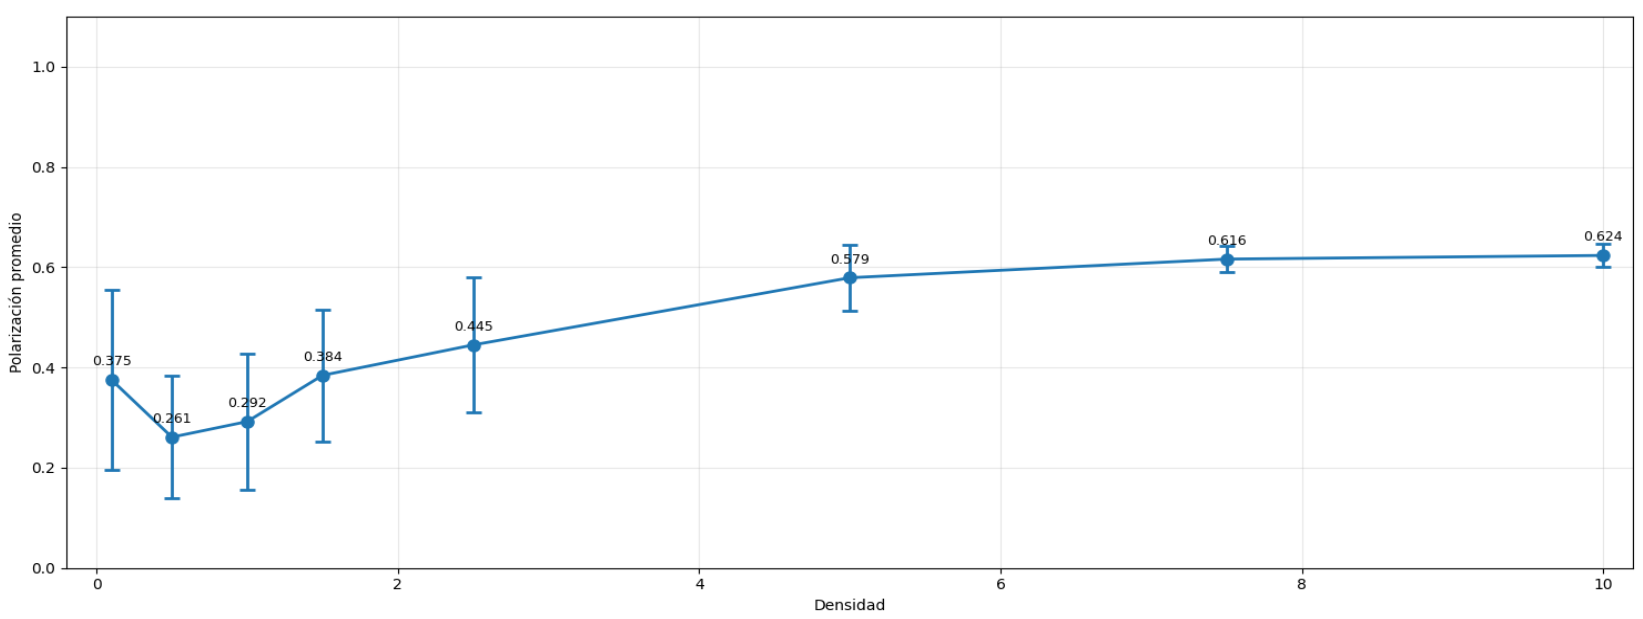
\includegraphics[width=0.9\textwidth]{20.png}
\caption{Valor promedio de la polarización en estado estacionario ($t = 250$) en función de la densidad $\rho$ para $\eta = 3$.}
\label{fig:20}
\end{figure}

Para el modelo clásico, los resultados muestran una transición de fase suave y continua en función del ruido $\eta$, consistente con lo reportado por Vicsek et al. [1]. A mayor densidad $\rho$, el sistema mantiene un orden notable incluso para valores de ruido más grandes, evidenciando el papel crucial de la densidad en la facilitación de interacciones.

\subsection{Modelo de Votante}
\subsubsection{Dependencia con el Ruido $\eta$}
\begin{figure}[H]
\centering
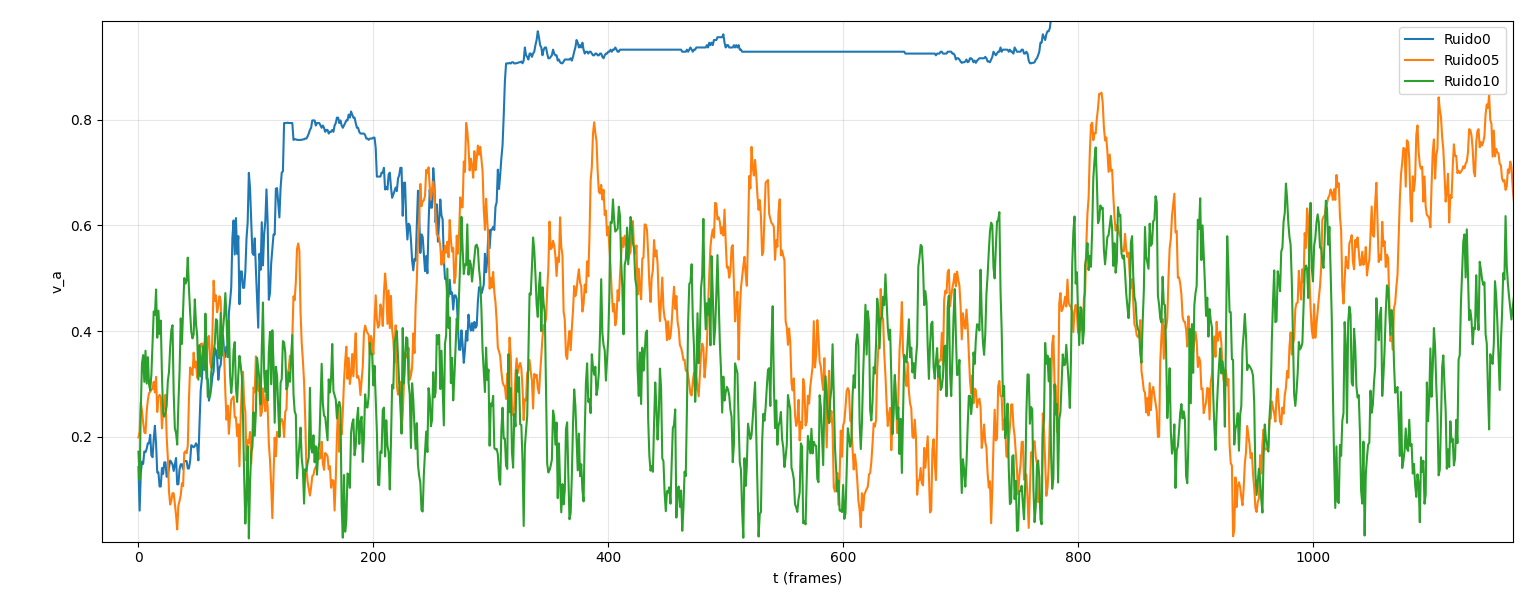
\includegraphics[width=0.9\textwidth]{Voter Densidad 0.5 Variando ruido.png}
\caption{Polarización $v_a$ en función del tiempo $t$ para el modelo de votante con $\rho = 0.5$ y $N = 50$, variando el ruido entre 0, 0.5 y 1.}
\label{fig:va_vs_eta_voter}
\end{figure}

\begin{figure}[H]
\centering
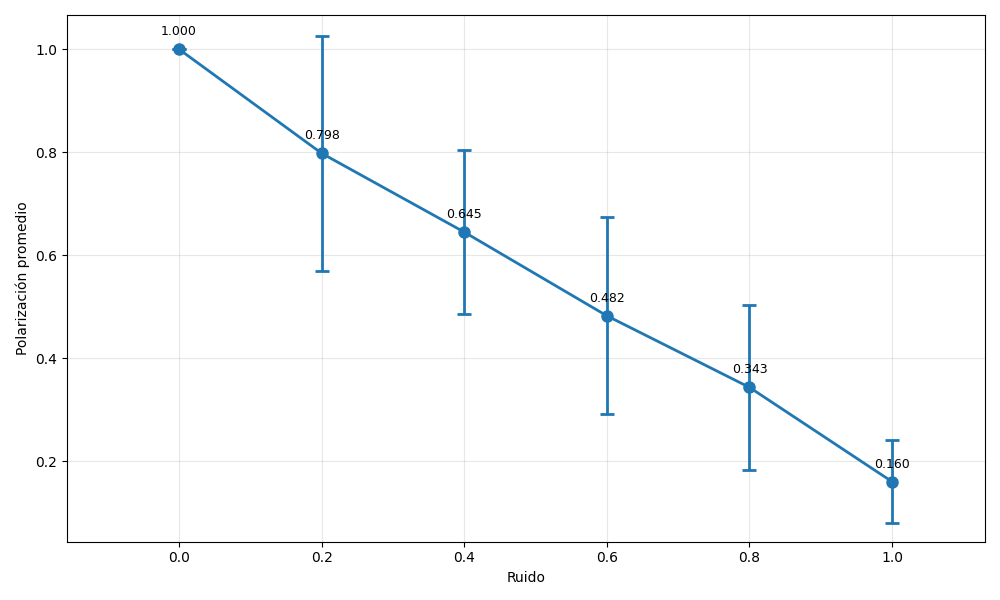
\includegraphics[width=0.9\textwidth]{Average voter dens 05 variando ruido.png}
\caption{Valor promedio de la polarización en estado estacionario ($t=800$) en función del ruido $\eta$ ($\rho = 0.5$, $N = 50$).}
\label{fig:promedio_va_eta_voter}
\end{figure}

\begin{figure}[H]
\centering
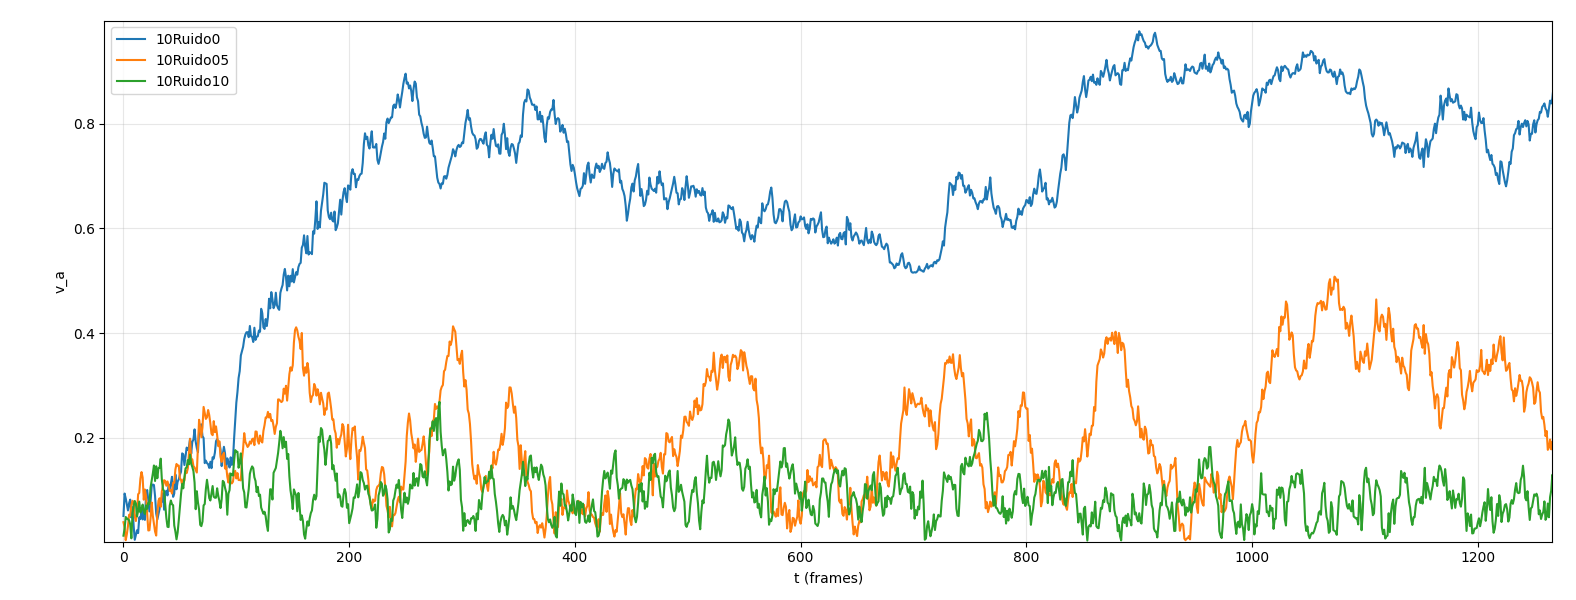
\includegraphics[width=0.9\textwidth]{Voter Densidad 10 Variando ruido.png}
\caption{Polarización $v_a$ en función del tiempo $t$ para el modelo de votante con $\rho = 10$ y $N = 1000$, variando el ruido $\eta$ entre 0, 0.5 y 1.}
\label{fig:va_vs_eta_voter2}
\end{figure}

\begin{figure}[H]
\centering
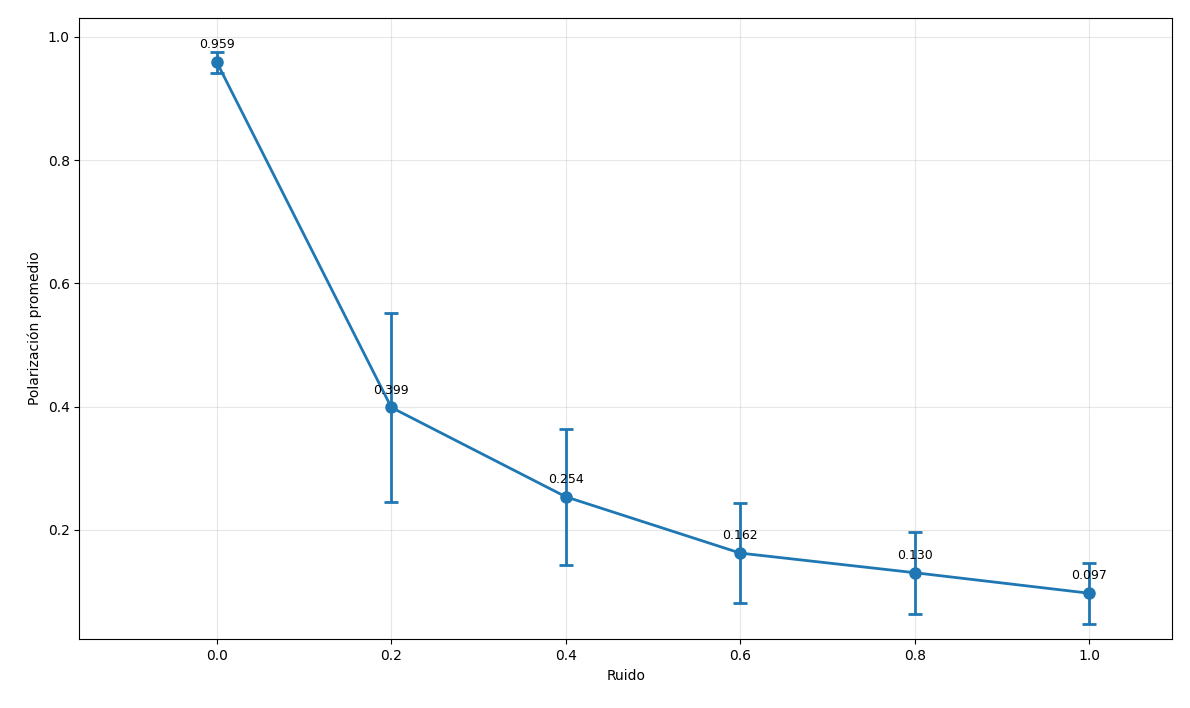
\includegraphics[width=0.9\textwidth]{Average voter dens 10 variando ruido.png}
\caption{Valor promedio de la polarización en estado estacionario ($t  = 800$) en función del ruido $\eta$ ($\rho = 10$, $N = 1000$).}
\label{fig:promedio_va_eta_voter2}
\end{figure}

\subsubsection{Dependencia con la Densidad $\rho$}

\begin{figure}[H]
\centering
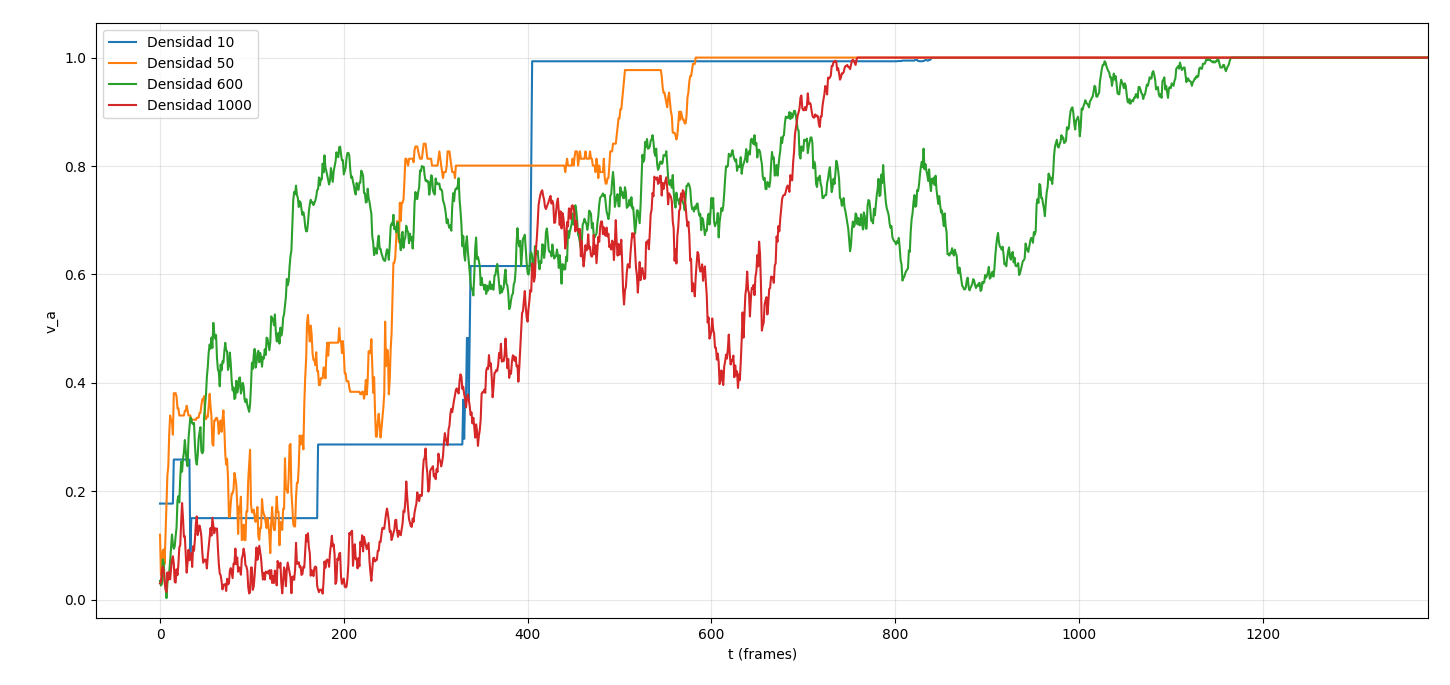
\includegraphics[width=0.9\textwidth]{Voter Ruido 0 variando densidad.png}
\caption{Polarización promedio en estado estacionario en función del tiempo $t$, con ruido $\eta = 0$, variando la densidad $\rho$ de partículas entre 0.1, 0.5, 6 y 10.}
\label{fig:promedio_va_densidad_voter0}
\end{figure}

\begin{figure}[H]
\centering
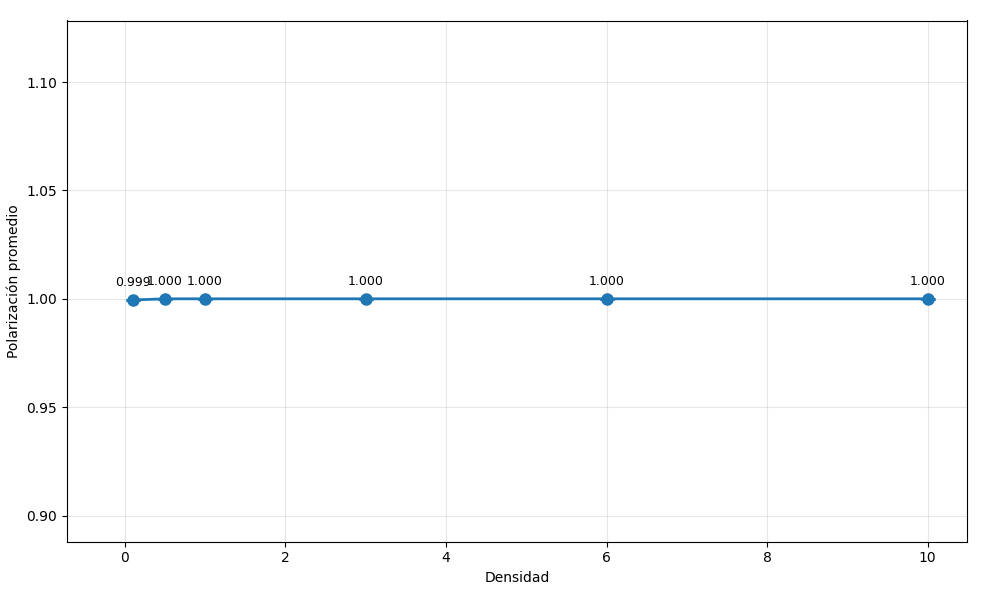
\includegraphics[width=0.9\textwidth]{Voter Ruido 0 variando densidad avg.png}
\caption{Valor promedio de la polarización en estado estacionario ($t  = 1200$) en función de la densidad $\rho$ ($\eta = 0$).}
\label{fig:va_tiempo_densidad_voter0}
\end{figure}

\begin{figure}[H]
\centering
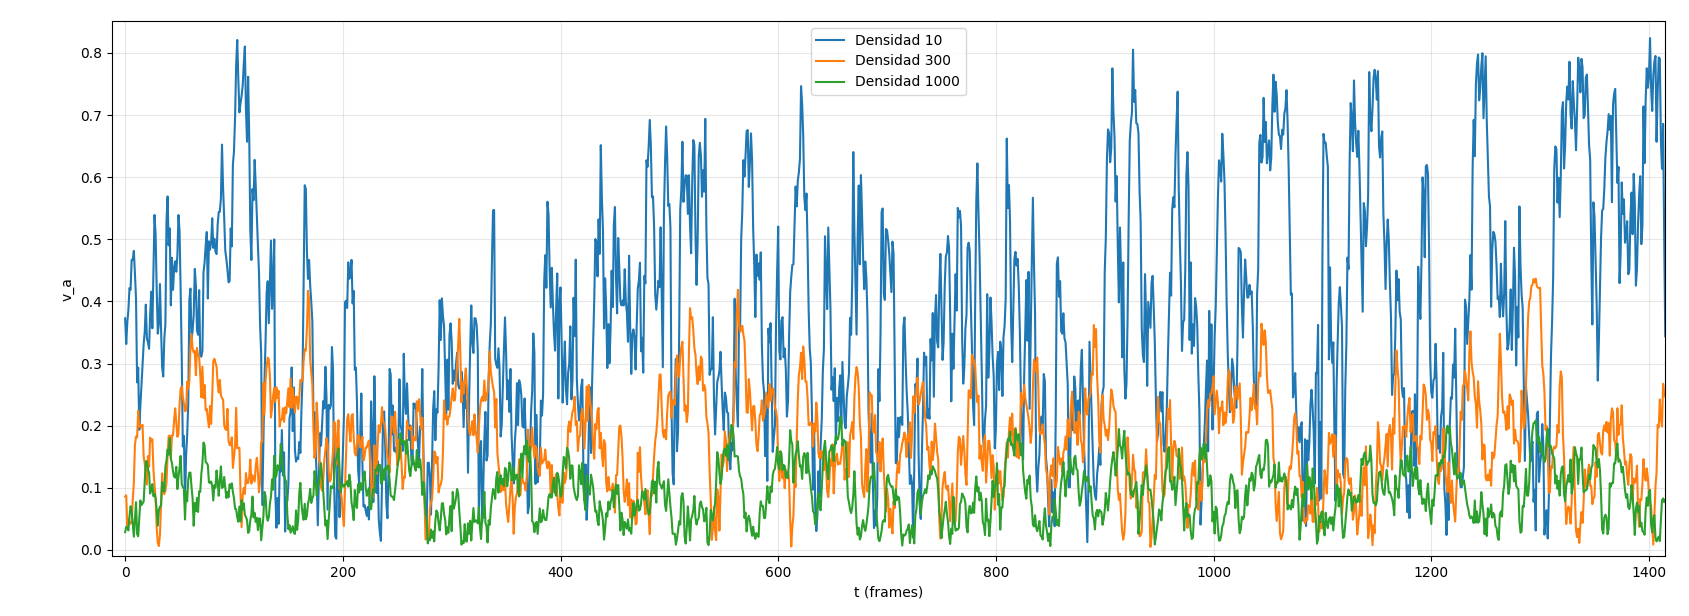
\includegraphics[width=0.9\textwidth]{Voter Ruido 1 variando densidad.png}
\caption{Polarización promedio en estado estacionario en función del tiempo $t$, con ruido $\eta = 1$, variando la densidad $\rho$ de partículas entre 0.1, 3 y 10.}
\label{fig:promedio_va_densidad_voter1}
\end{figure}

\begin{figure}[H]
\centering
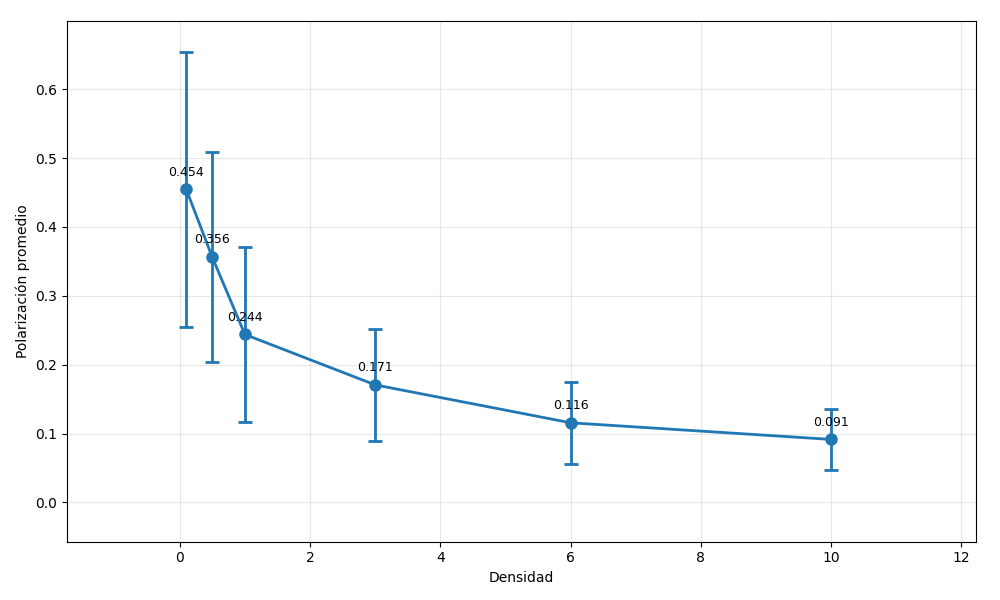
\includegraphics[width=0.9\textwidth]{Voter Ruido 1 variando densidad avg.png}
\caption{Valor promedio de la polarización en estado estacionario ($t  = 800$) en función de la densidad $\rho$ ($\eta = 1$).}
\label{fig:va_tiempo_densidad_voter1}
\end{figure}


El modelo de votante presenta un comportamiento cualitativamente diferente, con una transición más abrupta que ocurre a valores críticos de ruido más bajos ($\eta_c \approx 0.2$). Además, requiere densidades significativamente más altas para alcanzar el estado ordenado, reflejando la menor eficiencia del mecanismo de copia aleatoria individual.

\subsection{Análisis Comparativo}

La comparación entre ambos modelos revela que la naturaleza de las interacciones locales afecta profundamente las propiedades emergentes del sistema. Mientras el modelo clásico muestra una transición suave característica de sistemas con interacciones cooperativas extendidas, el modelo de votante exhibe una transición más abrupta típica de sistemas con dinámicas de consenso binario, consistente con lo reportado por Baglietto \& Vazquez [2].

\section{Conclusión}
A través de la implementación y análisis computacional de los modelos de Vicsek clásico y de votante, se logró caracterizar y comparar los fenómenos de ordenamiento colectivo en sistemas de partículas autopropulsadas. Los principales hallazgos de este trabajo son:

\begin{itemize}
    \item  Validación del modelo clásico: Reprodujimos exitosamente la transición de fase reportada por Vicsek (y otros), observando el paso de un estado desordenado ($v_a \approx 0$) a uno ordenado ($v_a \approx 1$) al disminuir el ruido $\eta$.

    \item Caracterización del modelo de votante: Implementamos y analizamos la variante propuesta por Baglietto \& Vazquez, encontrando una transición más abrupta que ocurre a valores críticos de ruido más bajos ($\eta_c \approx 0.2$).

    \item  Análisis comparativo: Demostramos que el mecanismo de interacción (promediado vs. copia aleatoria) altera cualitativamente la naturaleza de la transición de fase, siendo más suave en el modelo clásico y más abrupta en el modelo de votante.

    \item  Efecto de la densidad: Validamos que la densidad $\rho$ es un parámetro crucial que afecta la formación de la bandada, con mayores densidades favoreciendo el orden al facilitar las interacciones entre partículas.

    \item  Comportamiento emergente: Confirmamos que el orden global ($v_a$ alto) es una propiedad emergente que surge de interacciones locales simples entre partículas, sin un líder central.
\end{itemize}

En síntesis, este trabajo demostró exitosamente cómo reglas simples a nivel individual pueden generar comportamientos complejos y diversos a nivel macroscópico, y cómo la modificación de estos mecanismos de interacción altera fundamentalmente las propiedades colectivas del sistema.


\begin{thebibliography}{9}
\bibitem{vicsek} 
Vicsek, T., Czirók, A., Ben-Jacob, E., Cohen, I., \& Shochet, O. (1995). Novel type of phase transition in a system of self-driven particles. Physical review letters, 75(6), 1226.

\bibitem{baglietto} 
Baglietto, G., \& Vazquez, F. (2018). Flocking dynamics with voter-like interactions. Journal of Statistical Mechanics: Theory and Experiment, 2018(3), 033403.
\end{thebibliography}

\end{document}